\documentclass[openany]{article}
\usepackage[a4paper,margin=1in,bottom=1.5in]{geometry} % define margins. Bottom margin is used to lift a little bit the page number.
\usepackage[english]{babel} % document language is english
\usepackage{tikz} % for drawing (currently not used).
\usepackage{graphicx} % for including images
\usepackage[export]{adjustbox}
\usepackage{fancyhdr} % used for creating headers and footers. only used in title page in this document.
\usepackage{tabularx} % creation of more complex tables
\usepackage{longtable} % tables can span multiple pages
\usepackage{array} % allow elements of tabular environment to have vertical alignment, e.g., center alignment.
\usepackage{nameref} % make it possible to reference by name
\usepackage{hyperref} % allow hiperlinks (links to other document parts and extern links)
\usepackage{etoc} % used for generation of section local table of contents
\usepackage{placeins} % defines the \FloatBarrier command
\usepackage{siunitx} % SI units package
\usepackage{xcolor} % for modifying box color
\usepackage{adjustbox} % for modifying box parameters

% Define graphics path
\graphicspath{{figs/}}

% Configure the cross reference hyper links color
\hypersetup{
    colorlinks=true,
    linkcolor=blue,
}

\newcolumntype{C}{>{\centering\arraybackslash}X} % new column type for tabularx
						 % centered (\centering), adjust width in order to fill table width (X type)

% Configure header in 'titlepage'
\pagestyle{fancy}
\lhead{
\includegraphics[width=4.5cm]{logo_cnpem}}
\rhead{
\includegraphics[width=4cm]{logo_lnls}}
\renewcommand{\headrulewidth}{0pt}
\setlength{\headheight}{52pt}
% Clean footer
\fancyfoot{}

% increase table height factor a little bit (taller cells)
\renewcommand{\arraystretch}{1.5}

%==== Begin DOCUMENT ====
\begin{document}

%--- Begin title page ---
\begin{titlepage}

% Add header to this page
\thispagestyle{fancy}

% Center elements
\begin{center}

% title of title page
\topskip0pt % perfectly centered
\vspace*{\fill}
\textbf{\Huge DCCT EPICS Application User Guide}\\[20pt]
\textbf{\Huge Version 1.0}\\[20pt]
\textbf{\Huge June/2017}
\vspace*{\fill}

% footer of title page
\vfill
\textbf{Beam Diagnostics Group (DIG)}\\[5pt]
\textbf{Brazilian Synchrotron Light Laboratory (LNLS)}\\[5pt]
\textbf{Brazilian Center for Research in Energy and Materials (CNPEM)}
\end{center}

\end{titlepage}
%--- End of title page ---

\newpage
\pagestyle{plain} % restore default page style

%--- About this manual ---
\paragraph{}{\Large\bfseries About this manual}

\paragraph{} This manual provides an overview of the DCCT EPICS application. It is assumed that the reader is familiar with the basics of EPICS.

%--- Table of contents ---
\tableofcontents

\newpage
%--- Section: Introduction ---
\section{Introduction}

\paragraph{} The Direct-Current Current Transformer (DCCT) is the sensor responsible for measuring the beam average current. The DCCT application software is responsible for making DCCT measurements and configuration options available as EPICS Process Variables (PVs).

%--- Section: Instrument Setup ---
\section{Instrument Setup}

	\paragraph{} The complete DCCT measurement setup consists of a DCCT (Bergoz NPCT) mounted in the beam line; a digital multimeter (Kethley DMM7510) connected to the DCCT output terminals; a STD-EVE timing module, which has a multimeter trigger output connected to its rear panel and one of its front panel outputs connected to the multimeter trigger input; a PC which communicates with the digital multimeter.

	% Instrument Setup figure
	\begin{figure}[!h]
		\caption{Instrument Setup}
		\label{fig:dcct-setup}
		\centering
		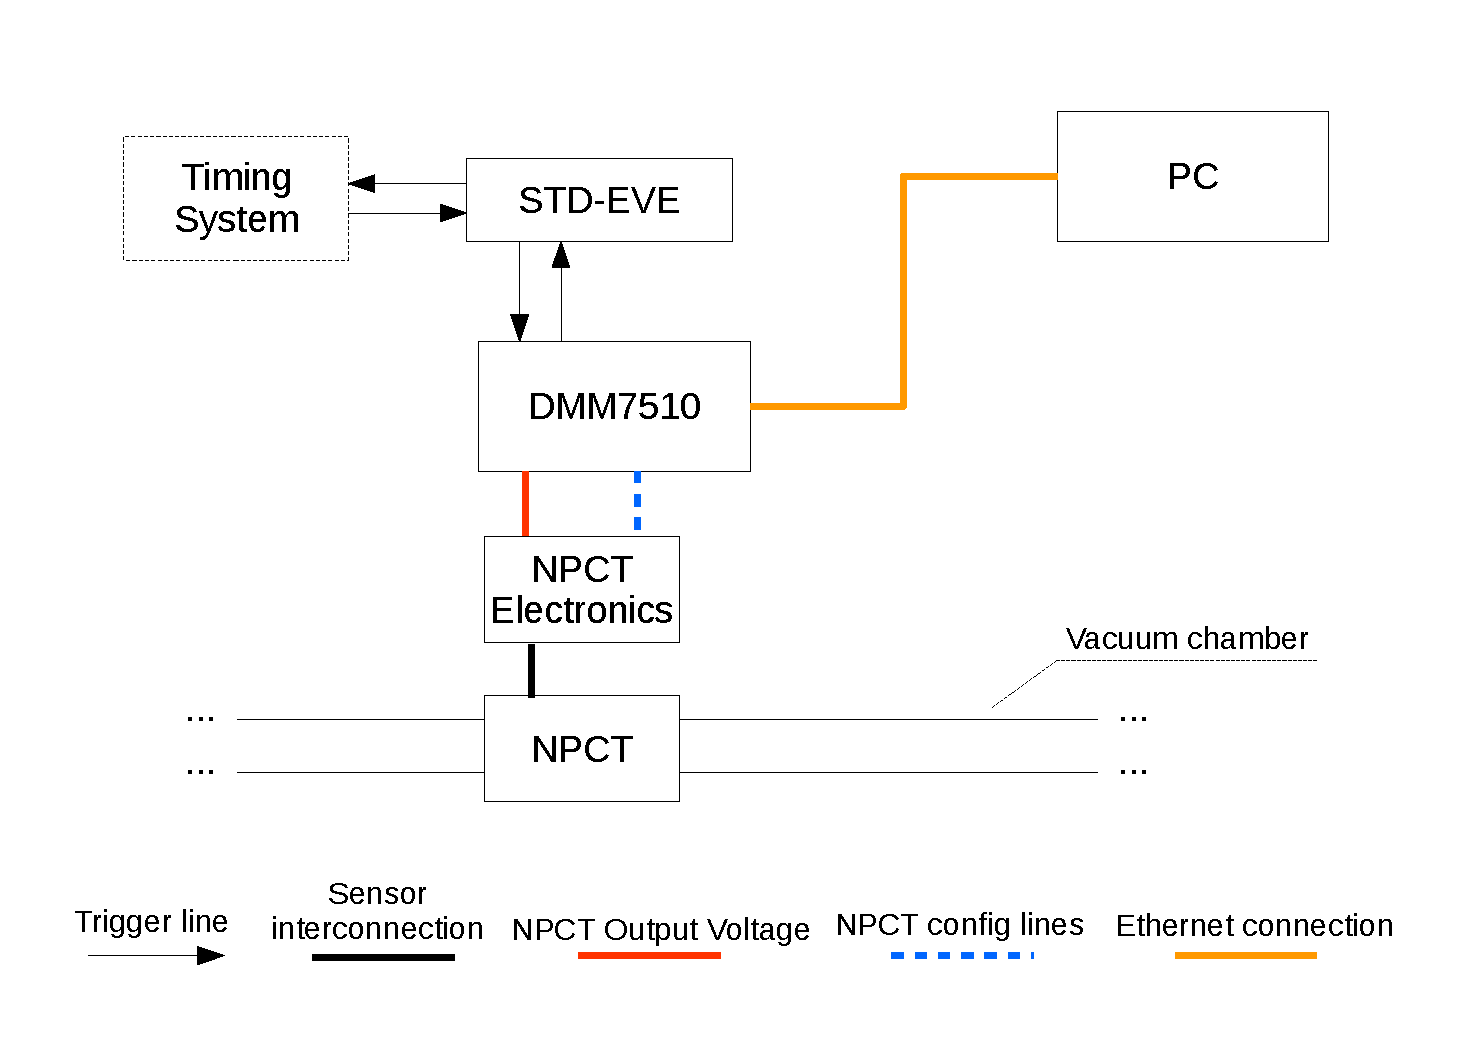
\includegraphics[width=1.0\textwidth]{dcct-setup-image}
	\end{figure}
\FloatBarrier

	\paragraph{} The NPCT (New Parametric Current Transformer) is a comercial DCCT, fabricated by Bergoz Instrumentation, widely used in particles accelerators around the world for measuring average beam current. The instrument generates a voltage output, in the 0 to 10 volts range, proportional to the current flowing through its toroid.

	\paragraph{} The Kethley DMM7510 digital multimeter is connected to the NPCT voltage output and is used to acquire, convert, and filter the sensor data. For the Storage Ring DCCT, the multimeter is also responsible for generating a trigger to the STD-EVE timing module whenever the current falls below a specified threshold, indicating that the beam has been lost.

	\paragraph{} The STD-EVE timing module can trigger multimeter readings, and monitor the multimeter output trigger line. Upon trigger reception, the STD-EVE generates a post-mortem event that is broadcast to the entire Timing System.

	\paragraph{} The PC runs an EPICS IOC, which includes DMM7510 multimeter and DCCT application-specific PVs. The application reads the multimeter data regularly and configures the multimeter's parameters according to the settings defined in the application PVs.

%--- Section: Measurement Overview ---
\section{Measurement Overview}

	\subsection{Storage Ring} 

		\paragraph{} Storage Ring beam current is measured periodically in fixed time steps. The measurement trigger can be provided by software, or by an external trigger pulse. When software triggering is selected, the DCCT application issues measurement commands at a 10 Hz rate. When external triggering is selected, the multimeter starts a measurement once an external trigger is received, which is provided by the Timing System. The most recent measurement is retrieved by the IOC at a rate of 5 Hz.

		\paragraph{} Another important task of the Storage Ring DCCT system is to inform the Timing System whenever the beam current falls below a minimum threshold. If configured to do so, the multimeter constantly monitors the DCCT output, comparing it to the specified threshold. When the current level falls below the threshold, the multimeter outputs a trigger pulse to the STD-EVE timing module in less than \SI{2}{\micro\second}.

	\subsection{Booster} 

		\paragraph{} Since, for the Booster, the beam current measurements must be correlated to each separate Booster ramp cycle, the timing of measurements is important. The measurement trigger in this application can be provided by an external trigger pulse, or by the beam current level itself. When in external trigger mode, the multimeter measurements are triggered by the STD-EVE module at each Booster ramp cycle. When triggered by current level, a measurement starts when the input signal becomes greater than the specified threshold. For both triggering modes, there is an user-configurable delay that can be used for better positioning the measurement start in the ramp cycle.

%--- Section: DCCT Software Configuration Steps ---
\section{DCCT Software Configuration}

	\paragraph{} This section describes the basic steps when configuring the DCCT application. Further detail about the DCCT application PVs can be found in \emph{\nameref{sec:process-variables}}.

	\bigskip
	\noindent\adjustbox{minipage=\textwidth,cfbox=red 1.0pt 2ex}{
		It is recommended that \hyperref[disable-triggering]{measurement triggering be disabled} before making any changes to the application settings and to configure triggering only after everything else has been set. This avoids incorrect measurements and/or false post-mortem signal generation.
	}

	\bigskip
	\noindent\adjustbox{minipage=\textwidth,cfbox=red 1.0pt 2ex}{A new \hyperref[relative-offset]{voltage relative offset} should be acquired every time the range configuration is modified.}

	\subsection{Measurement triggering}

		\paragraph{Disable triggering}\label{disable-triggering} It might be useful, in some cases, to disable measurement triggering. In this configuration, all trigger types are disabled.

			\begin{enumerate}
				\item Set \emph{MeasTrg-Sel} PV to \emph{None}.
				\item Wait until \emph{MeasTrg-Sts} has changed to \emph{None}.
			\end{enumerate}

		\paragraph{Software triggering} In the software triggering mode, the DMM7510 multimeter starts measurements in response to periodic software requests.

			\begin{enumerate}
				\item Set \emph{MeasTrg-Sel} PV to \emph{Software}.
				\item Wait until \emph{MeasTrg-Sts} has changed to \emph{Software}.
			\end{enumerate}

		\paragraph{External triggering} In the external triggering mode, the DMM7510 multimeter starts measurements in response to external trigger reception, while software periodic reads retrieve the newest measurement value available.

			\begin{enumerate}
				\item Set \emph{TrgDelay-SP} to the desired delay between trigger and measurement start.
				\item Verify if \emph{TrgDelay-RB} value is correct.
				\item Set \emph{MeasTrg-Sel} PV to \emph{External}.
				\item Wait until \emph{MeasTrg-Sts} has changed to \emph{External}.
			\end{enumerate}

		\paragraph{Current level based triggering} In level based triggering mode, the DMM7510 multimeter starts measurements in response to any beam current rising edge that goes above the specified threshold.

			\begin{enumerate}
				\item Set \emph{Range-Sel} to the desired DCCT sensor range.
				\item Verify if \emph{Range-Sts} has changed accordingly.
				\item Set \emph{Threshold-SP} to the current level threshold intended to trigger measurements.
				\item Verify if \emph{Threshold-RB} has changed accordingly.
				\item Set \emph{HFReject-Sel} to indicate if high frequency rejection should be used.
				\item Verify if \emph{HFReject-Sts} has changed accordingly.
				\item Set \emph{MeasTrg-Sel} to \emph{InLevel}.
				\item Wait until \emph{MeasTrg-Sts} has changed to \emph{InLevel}.
			\end{enumerate}

	\subsection{DCCT Range selection}

		\paragraph{} The selected DCCT sensor range should never be smaller than the current passing through the sensor. Currents exceeding the full scale range may saturate the sensor magnetic cores.

			\begin{enumerate}
				\item Set \emph{Range-Sel} to the desired DCCT sensor range.
				\item Verify if \emph{Range-Sts} has changed accordingly.
			\end{enumerate}

	\subsection{Low beam current detection}

		\paragraph{} Low beam current detection is used for post-mortem signal generation. \emph{This feature cannot be used along with current level based measurement triggering}.

			\begin{enumerate}
				\item Set \emph{Range-Sel} to the desired DCCT sensor range.
				\item Verify if \emph{Range-Sts} has changed accordingly.
				\item Set \emph{Threshold-SP} to the desired current level threshold.
				\item Verify if \emph{Threshold-RB} has changed accordingly.
				\item Set \emph{HFReject-Sel} to indicate if high frequency rejection should be used.
				\item Verify if \emph{HFReject-Sts} has changed accordingly.
				\item Set \emph{LowLimEnbl-Sel} to \emph{ON}.
				\item Verify if \emph{LowLimEnbl-Sts} status is \emph{ON}.
			\end{enumerate}

	\subsection{Measurement settings}

		% Measurement characteristcs figure 1
		\begin{figure}[!h]
			\caption{Measurement with Count=1, NPLC=2, LineSync=ON}
			\label{fig:meas-param1}
			\centering
			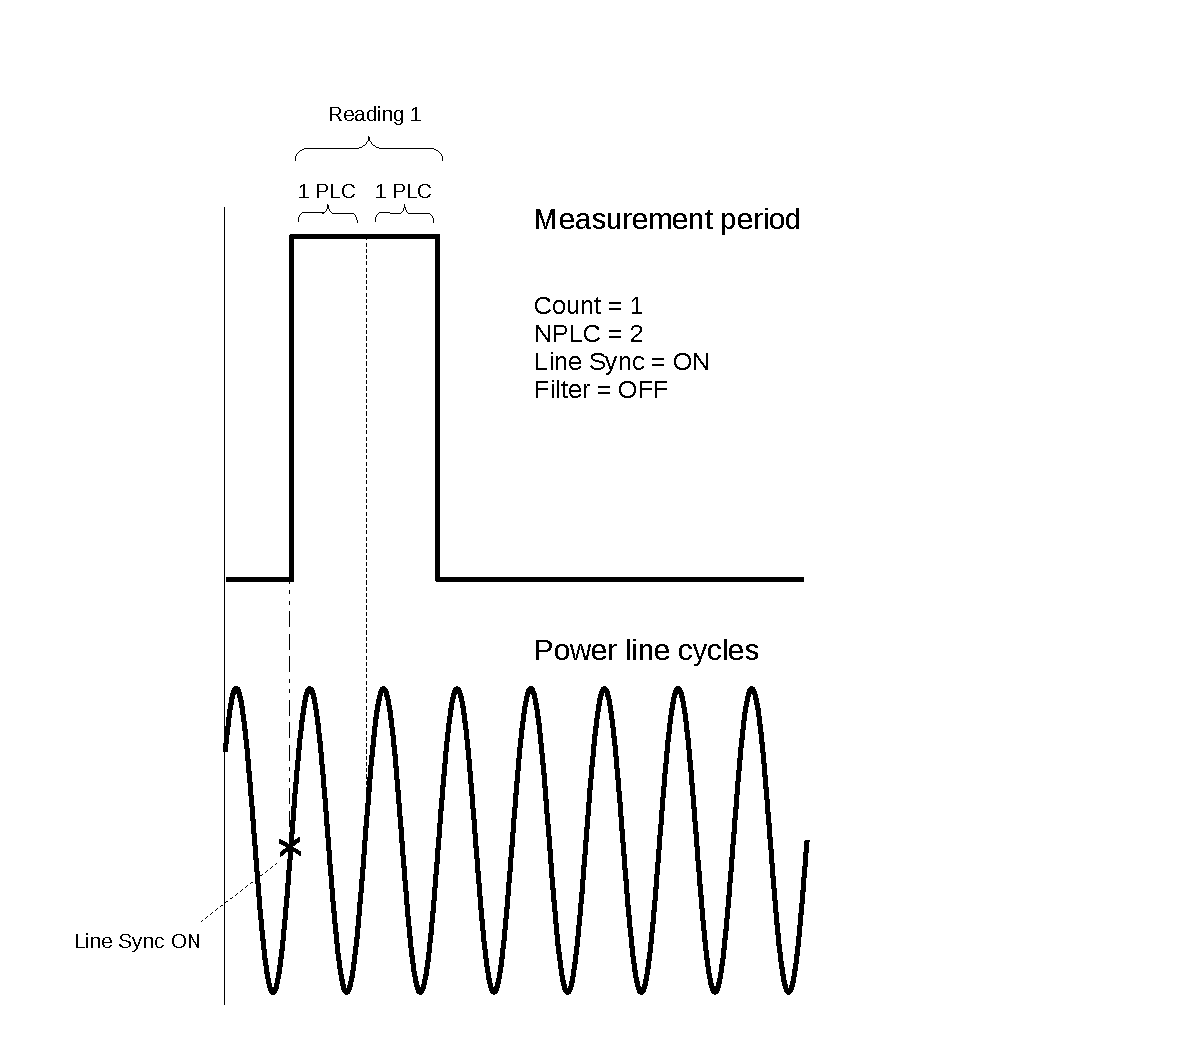
\includegraphics[width=1.0\textwidth]{dcct-meas-param1-image}
		\end{figure}

		% Measurement characteristcs figure 2
		\begin{figure}[!h]
			\caption{Measurement with Count=2, NPLC=2, LineSync=OFF}
			\label{fig:meas-param2}
			\centering
			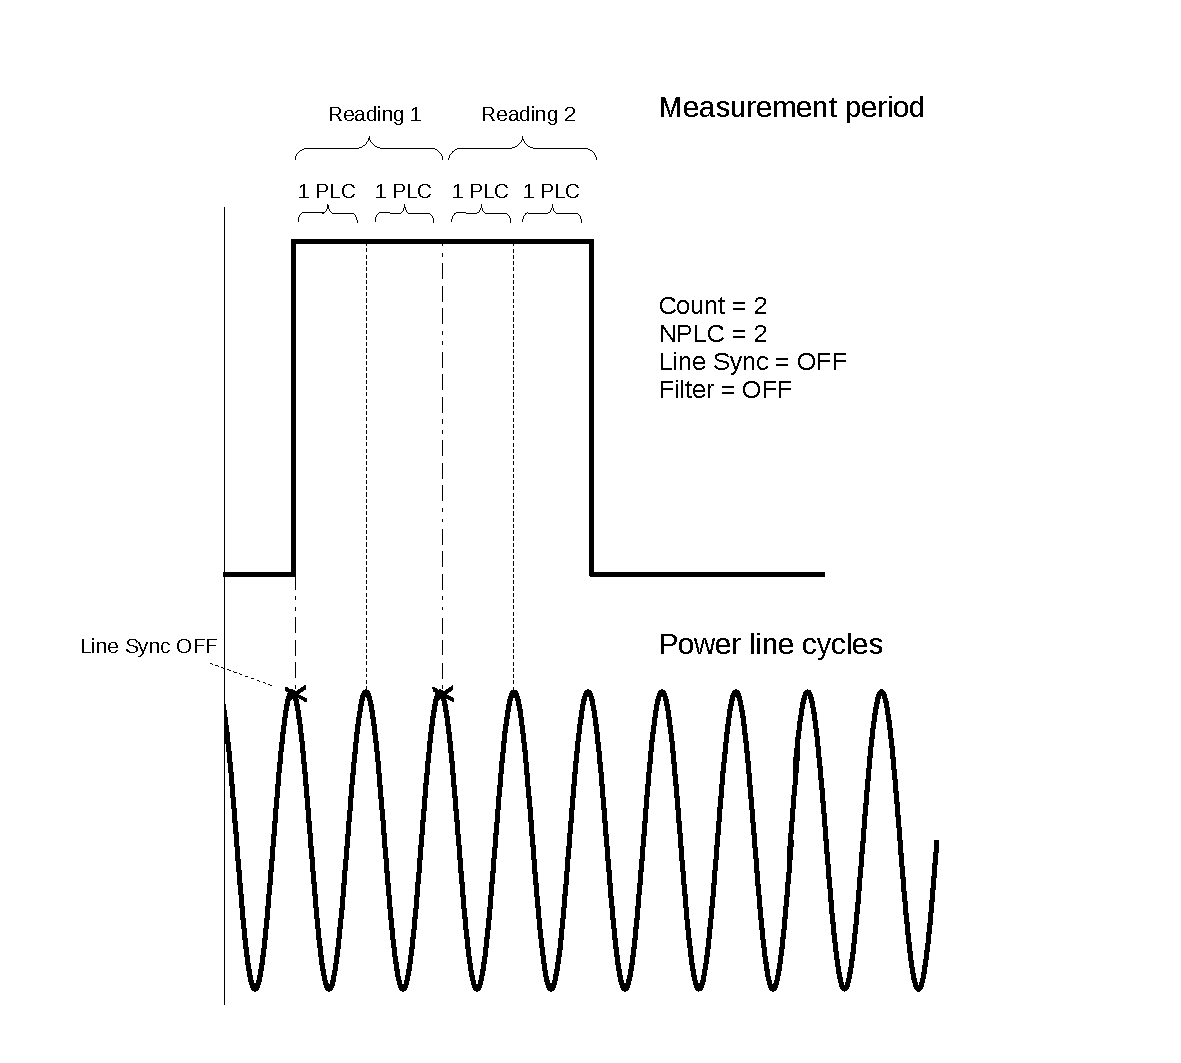
\includegraphics[width=1.0\textwidth]{dcct-meas-param2-image}
		\end{figure}

		% Measurement characteristcs figure 3
		\begin{figure}[!h]
			\caption{Measurement with Count=1, NPLC=2, FilterEnbl=ON, FilterCnt=3}
			\label{fig:meas-param3}
			\centering
			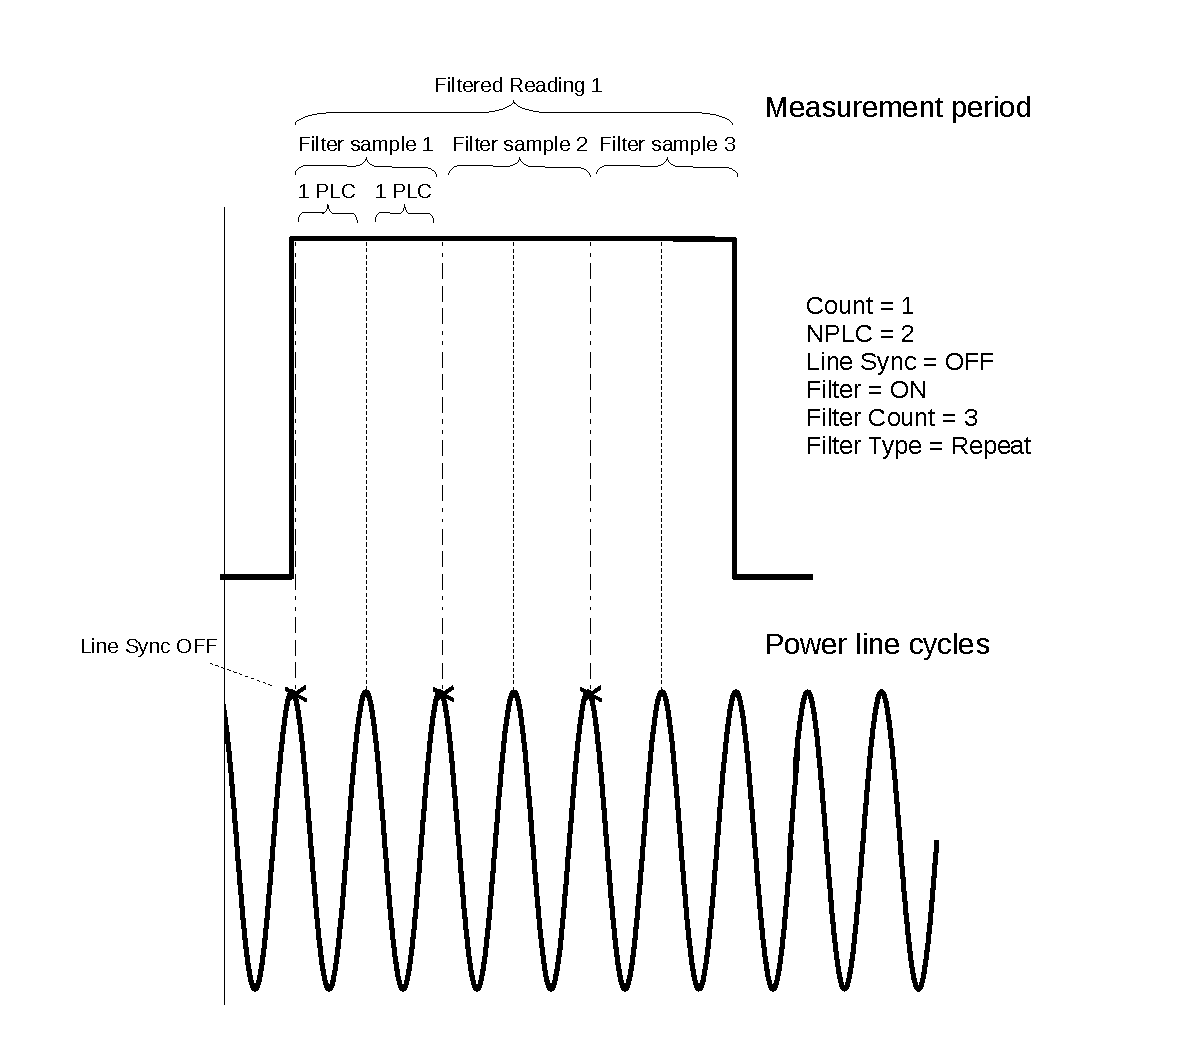
\includegraphics[width=1.0\textwidth]{dcct-meas-param3-image}
		\end{figure}
\FloatBarrier

		\paragraph{General} A few parameters are responsible for defining the measurement characteristics.

			\begin{enumerate}
				\item \emph{MeasCount-SP} sets the number of measurements per trigger. Only the latest measurement is retrieved by the software.
				\item \emph{MeasCount-RB} indicates the configured number of measurements per trigger.
				\item \emph{NPLC-SP} sets the measurement integration period in number of power line cycles.
				\item \emph{NPLC-RB} indicates the configured integration period in number of power line cycles.
				\item \emph{LineSync-Sel} sets if measurement integration period is synched to power line cycle zero crossing. Line synchronization affects measurement speed.
				\item \emph{LineSync-Sts} indicates the configured measurement power line synchronization status.
				\item \emph{Imped-Sel} sets the multimeter's input impedance. Recommended setting is \emph{AUTO}.
				\item \emph{Imped-Sts} indicates the configured multimeter's input impedance.
			\end{enumerate}

		\paragraph{Filter} It is possible to apply an averaging filter to measurements. If enabled, the specified number of samples are taken and averaged by the specified algorithm.

			\begin{enumerate}
				\item \emph{FilterCnt-SP} sets the number of measurements that are used to produce a reading.
				\item \emph{FilterCnt-RB} indicates the configured number of measurements used to produce reading.
				\item \emph{FilterTyp-Sel} sets the filter algorithm used.
				\item \emph{FilterTyp-Sts} indicates the configured filter algorithm.
				\item \emph{FilterWind-SP} sets the filter window. When a filter sample value exceeds the window threshold, the filter stack is filled immediately with that sample value.
				\item \emph{FilterWind-RB} indicates the filter configured window.
				\item \emph{FilterEnbl-Sel} enables/disables filtering.
				\item \emph{FilterEnbl-Sts} indicates the filter enable status.
			\end{enumerate}

		\paragraph{Relative offset}\label{relative-offset} The relative offset parameter is used to remove offsets caused by instrument zero drift.

			\begin{enumerate}
				\item \emph{RelLvl-SP} sets the relative offset voltage level. The offset is subtracted from the measured voltage before any conversion is performed.
				\item \emph{RelLvl-RB} indicates the configured relative offset voltage level.
				\item \emph{RelEnbl-Sel} enables/disables the relative offset.
				\item \emph{RelEnbl-Sts} indicates the relative offset enable status.
				\item \emph{RelAcq-Cmd} sets the relative offset level equal to the multimeter input voltage level.
			\end{enumerate}

	\subsection{DCCT calibration}

		\paragraph{} The DCCT has a test function which injects a +100mA test signal in the sensor head when enabled.

			\begin{enumerate}
				\item \emph{Test-Sel} enables/disables the DCCT calibration current.
				\item \emph{Test-Sts} indicates the DCCT calibration current enable status.
			\end{enumerate}

	\subsection{Save function}

		\paragraph{} The save function stores the current PV configurations and restore them when the IOC is restarted.

			\begin{enumerate}
				\item Set \emph{Save-Cmd} to \emph{ON} to cause the \emph{-SP} and \emph{-Sel} PVs' values to be saved. During IOC startup, the saved PV values are restored, recovering the previous configuration.
			\end{enumerate}

%--- Section: Reading Measurements from PVs ---
\section{Reading Measurements from PVs}

	\paragraph{} The DCCT measurement data is available in the following EPICS PVs.

		\begin{enumerate}
			\item \emph{AvgCurr-Mon} stores the latest current measurement.
			\item \emph{CurrHstr-Mon} is a circular buffer storing the last 1000 measurements.
		\end{enumerate}

\section{Process Variables Description}\label{sec:process-variables}

	% Process Variables description table
	\begin{longtable}{| m{3.0cm} m{4.5cm} m{7.0cm} |}
		\caption{Application Process Variables} \\ \hline
		\bfseries Name & \bfseries Data Type & \bfseries Description \label{tab:PV-description} \endfirsthead
		\caption{Application Process Variables} \\ \hline
		\bfseries Name & \bfseries Data Type & \bfseries Description \endhead \hline
		% --- row ---
		AvgCurr-Mon & FLOAT: 32-bit & \begin{tabular}{@{}m{6cm}@{}}
	    					Latest current measurement. This PV holds the latest measurement fetched from the multimeter.
						\end{tabular} \\ \hline
		% --- row ---
		CurrHstr-Mon & FLOAT[1000] & \begin{tabular}{@{}m{6cm}@{}}
	    					Last 1000 current measurements. This PV is a circular buffer holding the last 1000 current measurements.
						\end{tabular} \\ \hline
		% --- row ---
		MeasTrg-Sel & ENUM: None, External, InLevel, Software & \begin{tabular}{@{}m{6cm}@{}}
				      	  Measurement trigger source. When set to \emph{External}, the multimeter measurements are triggered by an external trigger. When set to \emph{InLevel}, measurements are triggered when the input signal exceeds the specified threshold (rising edge transition). For both \emph{External} and \emph{InLevel} triggering, the software fetchs priodically the latest reading stored in the multimeter's buffer. When set to \emph{Software}, measurements are requested periodically by software.
					  \end{tabular} \\ \hline
		% --- row ---
		MeasTrg-Sts & ENUM: Unknown, External, InLevel, Software, None & \begin{tabular}{@{}m{6cm}@{}}
	    					Trigger source selection status.
						\end{tabular} \\ \hline
		% --- row ---
		TrgDelay-SP & FLOAT: Min=0.000008, Max=100000 & \begin{tabular}{@{}m{6cm}@{}}
	    					Trigger delay. The trigger delay specifies, in seconds, the delay between the external or level based trigger and the measurement start.
						\end{tabular} \\ \hline
		% --- row ---
		TrgDelay-RB & FLOAT: Min=0.000008, Max=100000 & \begin{tabular}{@{}m{6cm}@{}}
	    					Trigger delay readback value.
						\end{tabular} \\ \hline
		% --- row ---
		Range-Sel & ENUM: 20 A, 2 A, 200 mA, 20 mA & \begin{tabular}{@{}m{6cm}@{}}
	    					DCCT range selection. The selected range must be large enough so that the current passing through the sensor does not exceed full scale range, in which case its magnetic cores may saturate.
						\end{tabular} \\ \hline
		% --- row ---
		Range-Sts & ENUM: 20 A, 2 A, 200 mA, 20 mA & \begin{tabular}{@{}m{6cm}@{}}
	    					DCCT range selection status.
						\end{tabular} \\ \hline
		% --- row ---
		LowLimEnbl-Sel & BOOL: OFF, ON & \begin{tabular}{@{}m{6cm}@{}}
	    					Enable/disable low beam current detection. When low current detection is enabled, whenever the beam current falls below the specified threshold (falling edge transition), the multimeter generates an output trigger pulse. \emph{Low current detection cannot be used along with level based triggering}.
						\end{tabular} \\ \hline
		% --- row ---
		LowLimEnbl-Sts & BOOL: OFF, ON & \begin{tabular}{@{}m{6cm}@{}}
	    					Low beam current detection enable status.
						\end{tabular} \\ \hline
		% --- row ---
		Threshold-SP & FLOAT: Min=0, Max=2000 & \begin{tabular}{@{}m{6cm}@{}}
	    					Current threshold. The current threshold value, specified in \SI{}{\milli\ampere}, used by low current detection or level based triggering.
						\end{tabular} \\ \hline
		% --- row ---
		Threshold-RB & FLOAT: Min=0, Max=2000 & \begin{tabular}{@{}m{6cm}@{}}
	    					Current threshold readback value.
						\end{tabular} \\ \hline
		% --- row ---
		HFReject-Sel & BOOL: OFF, ON & \begin{tabular}{@{}m{6cm}@{}}
	    					Enable/disable high frequency rejection. When enabled, high frequency rejection requires the signal to remain above or below the specified threshold, depending on the configuration, for at least \SI{64}{\micro\second} before a trigger is generated. This paremeter affects the low current level detection and the level based triggering.
						\end{tabular} \\ \hline
		% --- row ---
		HFReject-Sts & BOOL: OFF, ON & \begin{tabular}{@{}m{6cm}@{}}
	    					High frequency rejection enable status.
						\end{tabular} \\ \hline
		% --- row ---
		MeasCount-SP & LONG: Min=1, Max=1000000 & \begin{tabular}{@{}m{6cm}@{}}
	    					Measurement count. Number of measurements to perform upon trigger reception.
						\end{tabular} \\ \hline
		% --- row ---
		MeasCount-RB & LONG: Min=1, Max=1000000 & \begin{tabular}{@{}m{6cm}@{}}
	    					Measurement count readback value.
						\end{tabular} \\ \hline
		% --- row ---
		NPLC-SP & FLOAT: Min=0.0005, Max=15 & \begin{tabular}{@{}m{6cm}@{}}
	    					Number of power line cycles. Specifies the duration of the measurement integration period in number of power line cycles.
						\end{tabular} \\ \hline
		% --- row ---
		NPLC-RB & FLOAT: Min=0.0005, Max=15 & \begin{tabular}{@{}m{6cm}@{}}
	    					Number of power line cycles readback value.
						\end{tabular} \\ \hline
		% --- row ---
		LineSync-Sel & BOOL: OFF, ON & \begin{tabular}{@{}m{6cm}@{}}
	    					Enable/disable line synchronization. When line synchronization is enabled, measurement start is synched to positive slope zero crossings of power line cycles.
						\end{tabular} \\ \hline
		% --- row ---
		LineSync-Sts & BOOL: OFF, ON & \begin{tabular}{@{}m{6cm}@{}}
	    					Line synchronization enable status.
						\end{tabular} \\ \hline
		% --- row ---
		Imped-Sel & BOOL: AUTO, 10MOhm & \begin{tabular}{@{}m{6cm}@{}}
	    					Multimeter input impedance. Selecting \emph{AUTO} optimizes for low noise and charge injection when the device under test has less than \SI{100}{\kohm} input resistance. Otherwise, \emph{10MOhm} optimizes for lowest noise.
						\end{tabular} \\ \hline
		% --- row ---
		Imped-Sts & BOOL: AUTO, 10MOhm & \begin{tabular}{@{}m{6cm}@{}}
	    					Multimeter input impedance status.
						\end{tabular} \\ \hline
		% --- row ---
		FilterEnbl-Sel & BOOL: OFF, ON & \begin{tabular}{@{}m{6cm}@{}}
	    					Enable/disable filter. When filtering is enabled, the multimeter buffer readings are the result of different measurements averaged together using the specified algorithm.
						\end{tabular} \\ \hline
		% --- row ---
		FilterEnbl-Sts & BOOL: OFF, ON & \begin{tabular}{@{}m{6cm}@{}}
	    					Filter enable status.
						\end{tabular} \\ \hline
		% --- row ---
		FilterCnt-SP & LONG: Min=1, Max=100 & \begin{tabular}{@{}m{6cm}@{}}
	    					Filter count. Specifies the number of samples used to produce the filtered value, which is saved to the multimeter's buffer.
						\end{tabular} \\ \hline
		% --- row ---
		FilterCnt-RB & LONG: Min=1, Max=100 & \begin{tabular}{@{}m{6cm}@{}}
	    					Filter count readback value.
						\end{tabular} \\ \hline
		% --- row ---
		FilterTyp-Sel & BOOL: Repeat, Moving & \begin{tabular}{@{}m{6cm}@{}}
	    					Filter type selection. When set to \emph{Repeat}, a set of measurements are made and averaged together, resulting in the reading that is stored. When \emph{Moving} is selected, the measurements are made and continuously added to a FIFO of filter count length. Each time a new measurement is added to the FIFO, the FIFO elements' average produces a new filtered reading.
						\end{tabular} \\ \hline
		% --- row ---
		FilterTyp-Sts & BOOL: Repeat, Moving & \begin{tabular}{@{}m{6cm}@{}}
	    					Filter type status.
						\end{tabular} \\ \hline
		% --- row ---
		FilterWind-SP & LONG: Min=0, Max=10 & \begin{tabular}{@{}m{6cm}@{}}
	    					Filter window. Specifies the noise window size in percentage of range. The noise window allows a faster response to large signal changes. Readings that exceed the variation allowed by the window fills the filter stack immediately. Setting the filter window to \emph{0} disables the filter window.
						\end{tabular} \\ \hline
		% --- row ---
		FilterWind-RB & LONG: Min=0, Max=10 & \begin{tabular}{@{}m{6cm}@{}}
	    					Filter window readback value.
						\end{tabular} \\ \hline
		% --- row ---
		RelEnbl-Sel & BOOL: OFF, ON & \begin{tabular}{@{}m{6cm}@{}}
	    					Enable/disable relative offset. When relative offset is enabled, the relative offset level is subtracted from the readings raw value.
						\end{tabular} \\ \hline
		% --- row ---
		RelEnbl-Sts & BOOL: OFF, ON & \begin{tabular}{@{}m{6cm}@{}}
	    					Relative offset enable status.
						\end{tabular} \\ \hline
		% --- row ---
		RelLvl-SP & FLOAT: 32-bit & \begin{tabular}{@{}m{6cm}@{}}
	    					Relative offset level in volts. The level which is subtracted from readings raw value when relative offset is enabled.
						\end{tabular} \\ \hline
		% --- row ---
		RelLvl-RB & FLOAT: 32-bit & \begin{tabular}{@{}m{6cm}@{}}
	    					Relative offset level readback value.
						\end{tabular} \\ \hline
		% --- row ---
		RelAcq-Cmd & BOOL : OFF, ON & \begin{tabular}{@{}m{6cm}@{}}
						Acquire relative offset. Measure the multimeter voltage input and assign it to \emph{RelLvl-SP}. It is recommended that a new offset be acquired every time a new range is selected.
						\end{tabular} \\ \hline
		% --- row ---
		Test-Sel & BOOL: OFF, ON & \begin{tabular}{@{}m{6cm}@{}}
	    					Enable/disable DCCT test current. When enabled, injects a calibration current of +\SI{100}{\milli\ampere} to the sensor head.
						\end{tabular} \\ \hline
		% --- row ---
		Test-Sts & BOOL: OFF, ON & \begin{tabular}{@{}m{6cm}@{}}
 						DCCT test current enable status.
						\end{tabular} \\ \hline
		% --- row ---
		Save-Cmd & BOOL: OFF, ON & \begin{tabular}{@{}m{6cm}@{}}
 						Save command. When set to \emph{ON}, this PV causes all \emph{-SP} and \emph{-Sel} PVs values to be saved. During IOC initialization, the saved PV values are restored.
						\end{tabular} \\ \hline
		% --- row ---
		Download-Cmd & BOOL: OFF, ON & \begin{tabular}{@{}m{6cm}@{}}
 						Download command. When set to \emph{ON}, this PV causes all \emph{-SP} and \emph{-Sel} PVs' values to be transferred to hardware. This PV is set automatically during IOC initialization and when the IOC recovers from a communication problem with the hardware.
						\end{tabular} \\ \hline
	\end{longtable}

\end{document}
\grid
\grid
